\documentclass{beamer}
\usepackage{times, amsthm, amsmath, amssymb, cancel, changepage, graphicx, lipsum, fancyhdr, mathabx, enumitem,caption, subcaption}
\usetheme{CambridgeUS}
\usecolortheme{seagull}
\usefonttheme{serif}
\definecolor{navy}{RGB}{0, 0, 128} 
\setbeamercolor{frametitle}{fg=navy}
\setbeamercolor{title}{fg=navy}
\setbeamerfont{frametitle}{series=\bfseries}
\setbeamerfont{title}{series=\bfseries}



\title{Lecture 8: Optimization}
\date{September 19, 2019}

\begin{document}
	
\frame{\titlepage}


\begin{frame}
\frametitle{Optimization}
\begin{figure}
	\centering
	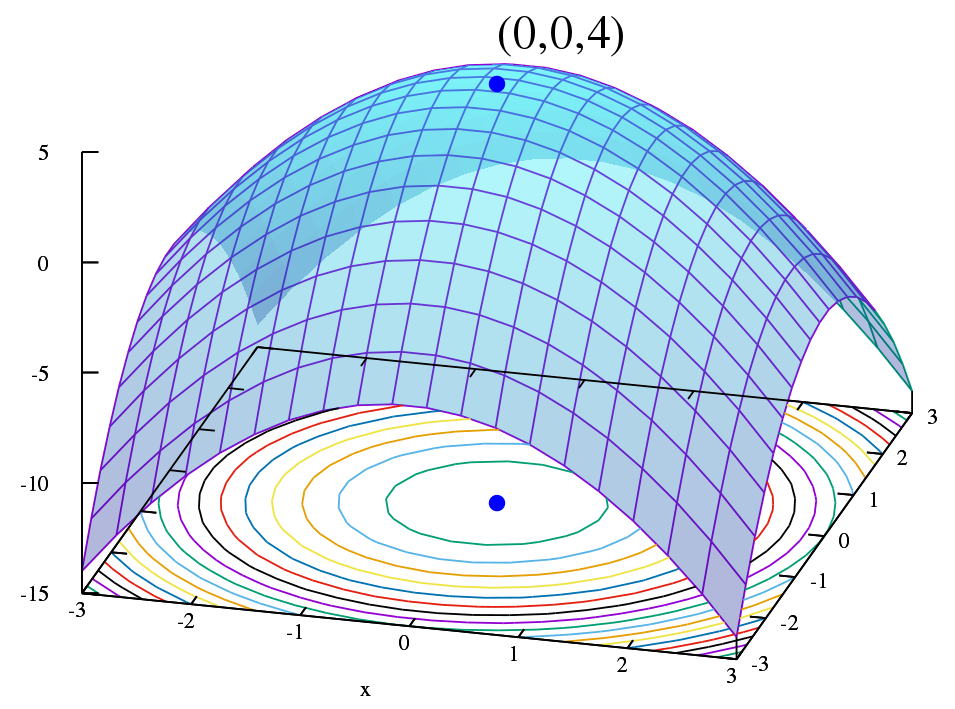
\includegraphics[height=.5\textheight]{maxpoint.png}\\
	\hspace*{10pt}\hbox{\thinspace{\tiny\itshape Wikipedia}}
\end{figure}

One of the main application of derivatives is finding a maximum or minimum. We discussed this using one variable, and similar concepts apply. Optimization deals with finding max or min points subject to some constraint.
\end{frame}


\begin{frame}
\frametitle{Maximums \& Minimums}
A function of two variables has a local maximum at $(a,b)$ if $f(x,y) \leq f(a,b)$ for all $(x,y)$ in some disk with center $(a,b)$. $f(a,b)$ is then the local maximum. If $f(x,y) \geq f(a,b)$ on such a disk, $f(a,b)$ is the local minimum.\\
\textit{Note: If the inequalities hold on the entire domain of $f(x,y)$ then we have a global max or min.}
\begin{itemize}
	\item[(i)] If $f$ has a local extrema at $(a,b)$ and the 1st partial derivative exists, then 
	$$\frac{\partial f}{\partial x} (a,b) = 0, \mbox{ and } \frac{\partial f}{\partial y} (a,b) = 0$$
	\item[(ii)] A point $(a,b)$ where all existing partial derivatives equals zero is called a critical or stationary point.
	\item[(iii)] A critical point is not necessarily an extrema of $f$. A critical point can be a max, min, or saddle point.
\end{itemize}
 
\vspace{6pt}
\textbf{Examples:}
\begin{itemize}
	\item[(a)] $f(x,y) = x^2+y^2 -2x -6y + 14$
	\item[(b)] $f(x,y) = y^2-x^2$
\end{itemize}
\end{frame}

\begin{frame}
\frametitle{Second Derivative Test for Extrema}
To test whether a critical point is a max, min, or saddle calculate $D$ where
$$D(a,b) = f_{xx}(a,b)f_{yy}(a,b) - [f_{xy}(a,b)]^2$$
\begin{itemize}
	\item -If $D>0$ and $f_{xx}(a,b) > 0$ then $f(a,b)$ is a local min.
	\item -If $D>0$ and $f_{xx}(a,b) < 0$ then $f(a,b)$ is a local max.
	\item -If $D<0$ then $f(a,b)$ is a saddle point.
	\item -If $D=0$ then the test fails.
\end{itemize}

\vspace{6pt}
\textbf{Examples:}
\begin{itemize}
	\item[(a)] $f(x,y) = x^2-y^2$
	\item[(b)] $f(x,y) = x^2-xy + y^2$
\end{itemize}
\end{frame}

\begin{frame}
\frametitle{Finding Extreme Values}
\begin{theorem}[Extreme Value Theorem]
	If $f(x,y)$ is continuous on a closed bounded set $D$ in $\mathbb{R}^2$, then $f$ attains an absolute min value $f(a_1,b_1)$ and also a max value $f(a_2,b_2)$ at some points $(a_1,b_1)$ and $(a_2,b_2)$ in $D$ such that
	$$f(a_1,b_1) \leq f(x,y) \leq f(a_2,b_2)$$
\end{theorem}

To find the absolute extrema of a continuous function on a closed, bounded $D$:
\begin{itemize}
	\item[(i)] Find the values of $f$ at the critical points of $f$ in $D$.
	\item[(ii)] Find the extreme values of $f$ on the boundary of $D$.
\end{itemize}

\vspace{6pt}
\textbf{Examples:}\\
\begin{itemize}
	\item[(a)] $f(x,y) = 1+x^2+y^2$
	\item[(b)] $f(x,y) = 5-3x+4y$ on closed triangle with vertices $(0,0)$, $(4,0)$, $(4,5)$.
\end{itemize}
\end{frame}


\begin{frame}
\frametitle{Lagrange Multipliers}
Suppose we want to minimize $f(x,y)$ subject to constraint $g(x,y)=0$. Then we use $F=f(x,y) + \lambda g(x,y)$ and solve the following system of equations:
\begin{eqnarray*}
	\frac{\partial F}{\partial x} &=& 0\\
	\frac{\partial F}{\partial y} &=& 0\\
	\frac{\partial F}{\partial \lambda} &=& 0
\end{eqnarray*}

\vspace{6pt}
\textbf{Examples:}
\begin{itemize}
	\item[(a)] Minimize $f(x,y) = (x-1)^2 +y^2$ subject to $y^2=4x$
	\item[(b)] Minimize $f(x,y) = x^2-y^2$ subject to $x^2+y^2 = 1$
	\item[(c)] Minimize $f(x,y) = x^2 + y$ subject to $x^2+y^2 = 1$
	
\end{itemize}
\end{frame}



%\begin{frame}
%\frametitle{What is a Limit?}
%\begin{figure}
%	\centering
%	\begin{subfigure}{0.48\textwidth}
%		
%		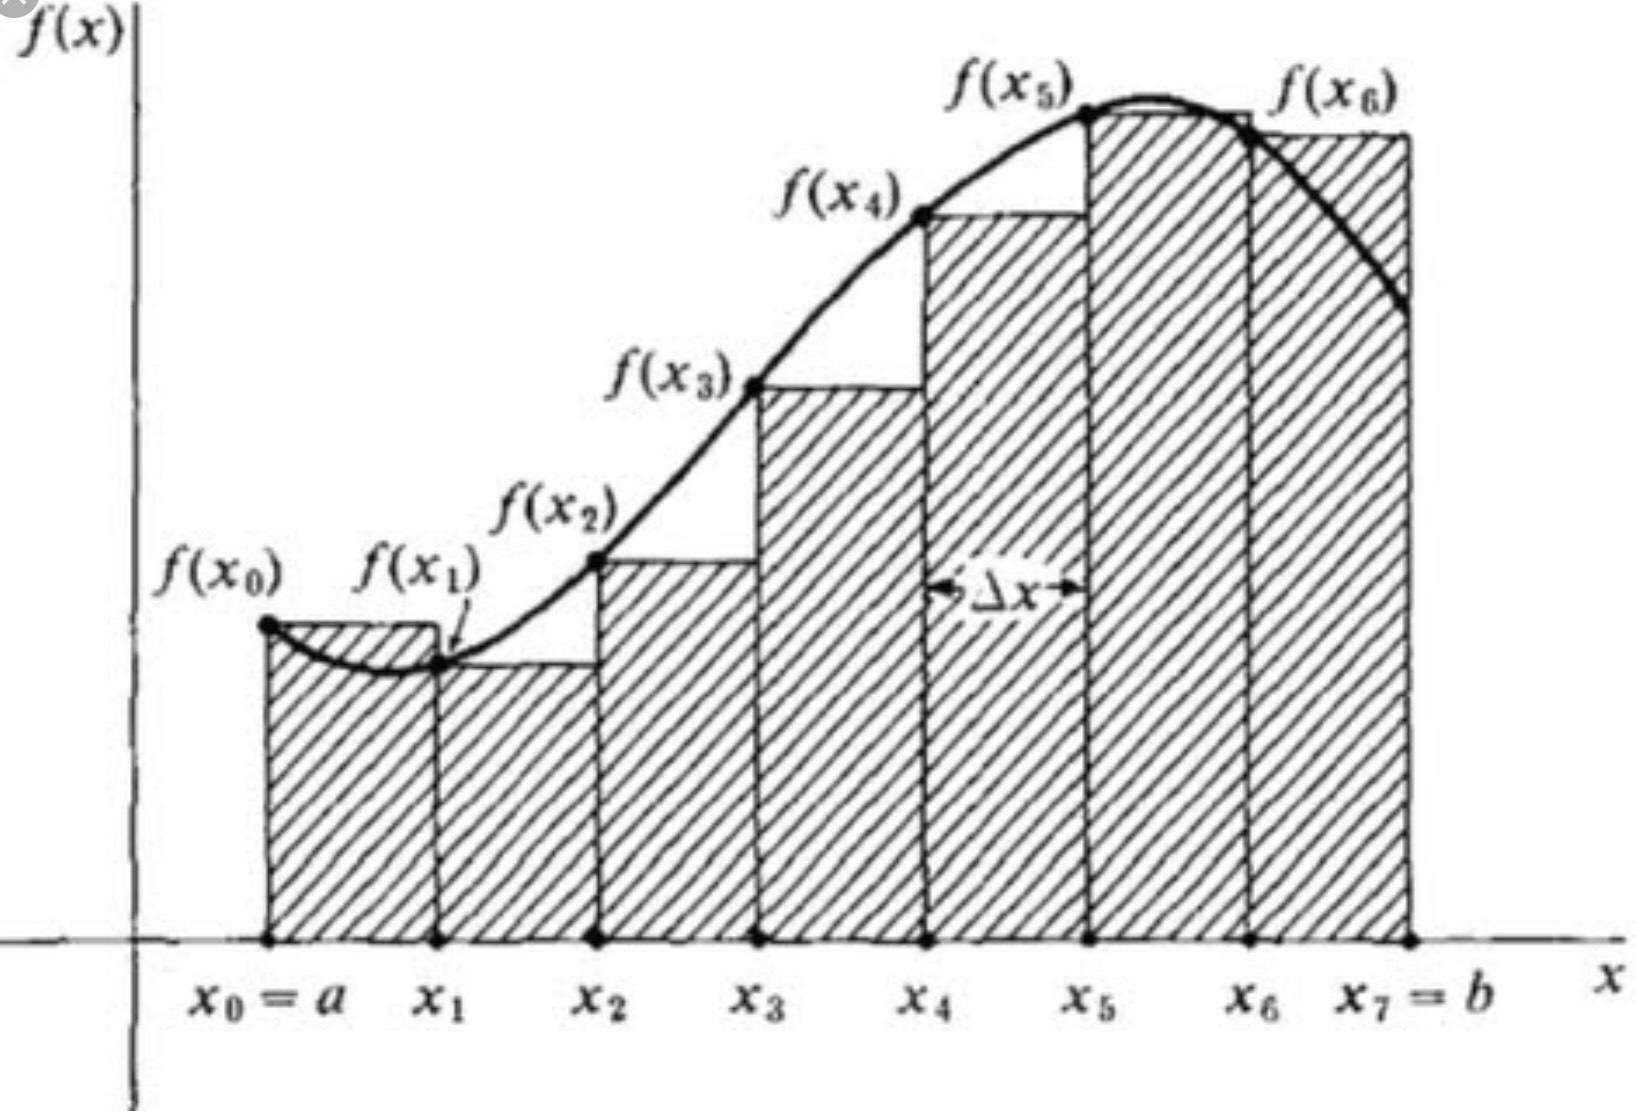
\includegraphics[width=\textwidth]{IMG_0380.jpg}
%		\hspace*{10pt}\hbox{\thinspace{\tiny\itshape vias.org}}
%		\caption{Single integration}
%	\end{subfigure}% 
%	~ 
%	\begin{subfigure}{0.48\textwidth}
%		
%		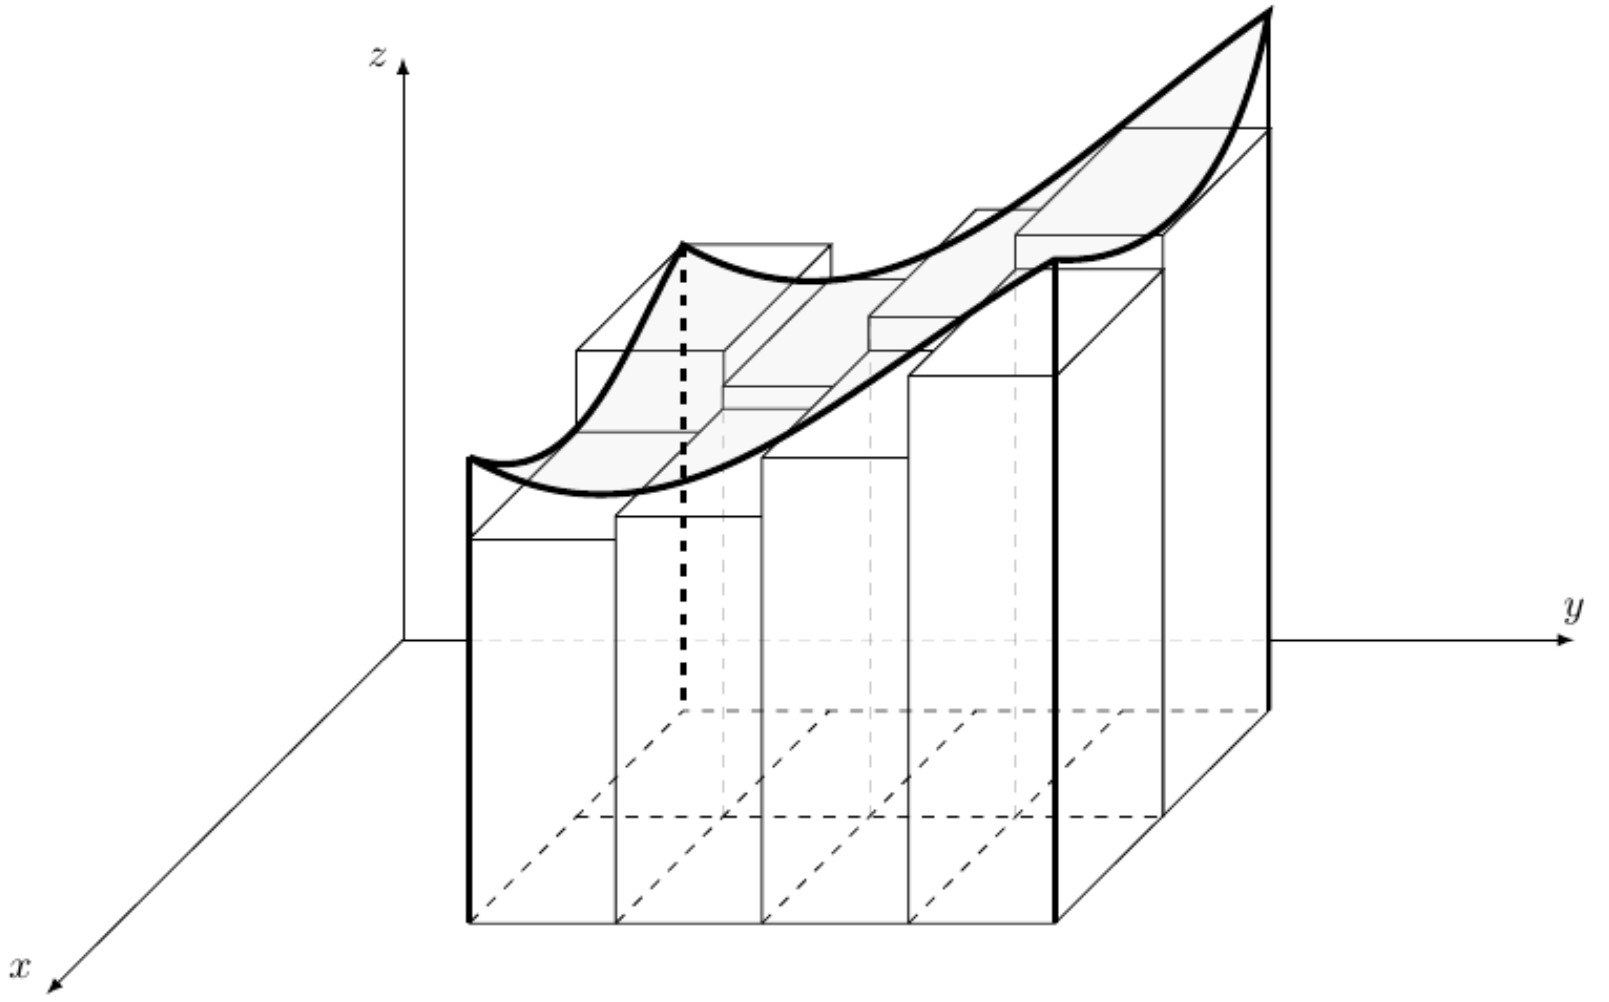
\includegraphics[width=\textwidth]{IMG_0385.jpg}
%		\hspace*{10pt}\hbox{\thinspace{\tiny\itshape tex.stackexchange.com}}
%		\caption{Double integration.}
%		\label{fig:2}
%	\end{subfigure}
%\end{figure}
%
%\end{frame}
%
%
%\begin{frame}
%\frametitle{Triple Integral}
%\begin{figure}
%	\centering
%	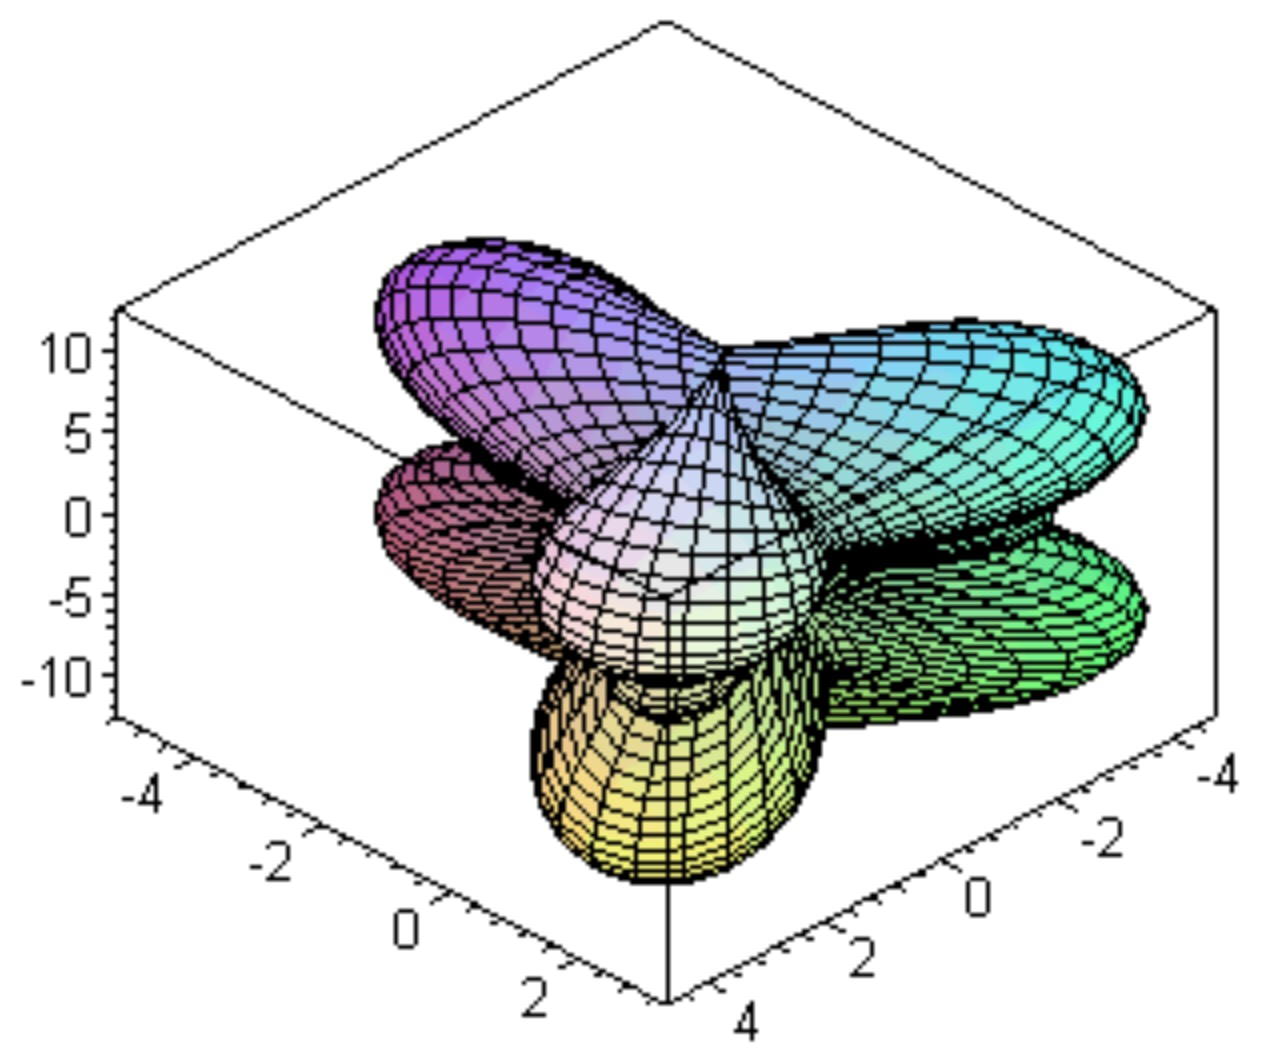
\includegraphics[height=.45\textheight]{IMG_0384.jpg}\\
%	\hspace*{10pt}\hbox{\thinspace{\tiny\itshape maplesoft.com}}
%\end{figure}
%
%$$\iiint\limits_{\mathbb{R}} F(x,y,z) dV = \int_{x=a}^{x=b} \int_{y=y_1(x)}^{y=y_2(x)} \int_{z=z_1(x,y)}^{z=z_2(x,y)} F(x,y,z) dz\,dy\,dx$$
%\textbf{Example:}
%\begin{itemize}
%	\item[(a)] $\int_0^1 \int_0^{1-x} \int_0^{2-x} xyz \,dz\,dy\,dx$
%\end{itemize}
%\end{frame}

\end{document}
